\chapter{Appendix}
\section{Schlick's approximation}
The Fresnel's equations describe the reflection and transmission of electromagnetic waves at an interface. That is, they give the reflection and transmission coefficients for waves parallel and perpendicular to the plane of incidence. Schlick's approximation is a formula for approximating the contribution of the Fresnel term where the specular reflection coefficient $R$ can be approximated by:

\begin{equation}
 R(\theta) = R_0 + (1 - R_0)(1 - \cos \theta)^5
\label{eq:schlickapprox}
\end{equation}

and

\begin{equation*}
  R_0 = \left(\frac{n_1-n_2}{n_1+n_2}\right)^2
\end{equation*}

where $\theta$ is the angle between the viewing direction and the half-angle direction, which is halfway between the incident 
light direction and the viewing direction, hence $\cos\theta=(H\cdot V)$. And $n_1,\,n_2$ are the indices of refraction of the two medias at the interface and $R_0$ is the reflection coefficient for light incoming parallel to the normal (i.e., the value of the Fresnel term when $\theta = 0$ or minimal reflection). In computer graphics, one of the interfaces is usually air, meaning that $n_1$ very well can be approximated as 1.

\section{Spherical Coordinates}
\label{sec:sphericalcoordinates}
$\forall \colvec[x]{y}{z} \in \mathbb{R}^3 : \exists r \in [0,\infty) \exists \phi \in [0,2\pi] \exists \theta \in [0,\pi] $ s.t.
\begin{equation*}
\colvec[x]{y}{z} = \colvec[r sin(\theta)cos(\phi)]{r sin(\theta)sin(\phi)}{r cos(\theta)}
\label{eq:sphericalcoordinates}
\end{equation*}


\section{Tangent Space}
\label{sec:tangentspace}
The concept of tangentspace-transformation of tangent space is used in order to convert a point between world and tangent space. GLSL fragment shaders require normals and other vertex primitives declared at each pixel point, which mean that we have one normal vector at each texel and the normal vector axis will vary for every texel. 

Think of it as a bumpy suface defined on a flat plane. If those normals were declared in the world space coordinate system, we would have to rotate these normals every time the model is rotated, even when just for a small amount. Since the lights, cameras and other objects are usually defined in world space coordinate system, and therefore, when they are involved in an calculation within the fragment shader, we would to have to rotate them as well for every pixel. This would involve almost countless many object to world matrix transformations meed to take place at the pixel level. Therefore, instead doing so, we transform all vertex primitives into tangent space within the vertex shader. 

To make this point clear an example: Even we would rotate the cube in figure $\ref{fig:cubeintangentspace}$, the tangent space axis will remain aligned with respect to the face. Which practically speaking, will save us from performing many space transformations applied pixel-wise within the fragment shader and instead allows us to perform us the tangenspace transformation of every involved vertex primitive in the vertex-shader.

\begin{figure}[H]
  \centering
  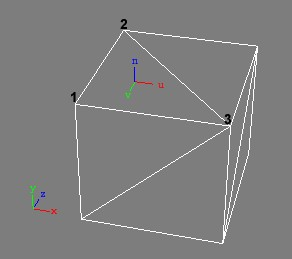
\includegraphics[scale=0.8]{background/cubeintangentspace.jpg}
  \caption{Cube in world space $(x,y,z)$ showing the tangen space $(u,v,n)$ of its face $(2,1,3)$}
  \label{fig:cubeintangentspace}
\end{figure}






